\documentclass[
10pt,
a4paper,
oneside,
headinclude,footinclude,
BCOR5mm,
]{article}

\usepackage[
nochapters, % Turn off chapters since this is an article        
beramono, % Use the Bera Mono font for monospaced text (\texttt)
eulermath,% Use the Euler font for mathematics
pdfspacing, % Makes use of pdftex’ letter spacing capabilities via the microtype package
dottedtoc % Dotted lines leading to the page numbers in the table of contents
]{classicthesis} % The layout is based on the Classic Thesis style

\usepackage{arsclassica} % Modifies the Classic Thesis package
\usepackage[T1]{fontenc} % Use 8-bit encoding that has 256 glyphs
\usepackage[utf8]{inputenc} % Required for including letters with accents
\usepackage{graphicx} % Required for including images
%% \graphicspath{{Figures/}} % Set the default folder for images
\usepackage{enumitem} % Required for manipulating the whitespace between and within lists
\usepackage{lipsum} % Used for inserting dummy 'Lorem ipsum' text into the template
\usepackage{subfig} % Required for creating figures with multiple parts (subfigures)
\usepackage{amsmath,amssymb,amsthm} % For including math equations, theorems, symbols, etc
\usepackage{varioref} % More descriptive referencing
\usepackage{geometry}
\usepackage{float}

\geometry{
  a4paper,
  total={170mm,257mm},
  left=20mm,
  top=20mm,
}

%----------------------------------------------------------------------------------------
%	COMMANDS
%---------------------------------------------------------------------------------------
\newcommand{\TSP}{\textit{Travelling Salesman Problem}}
\newcommand{\GO}{\texttt{Go }}


%----------------------------------------------------------------------------------------
%	THEOREM STYLES
%---------------------------------------------------------------------------------------

\theoremstyle{definition} % Define theorem styles here based on the definition style (used for definitions and examples)
\newtheorem{definition}{Definition}

\theoremstyle{plain} % Define theorem styles here based on the plain style (used for theorems, lemmas, propositions)
\newtheorem{theorem}{Theorem}

\theoremstyle{remark} % Define theorem styles here based on the remark style (used for remarks and notes)

%----------------------------------------------------------------------------------------
%	HYPERLINKS
%---------------------------------------------------------------------------------------

\hypersetup{
%draft, % Uncomment to remove all links (useful for printing in black and white)
colorlinks=true, breaklinks=true, bookmarks=true,bookmarksnumbered,
urlcolor=webbrown, linkcolor=RoyalBlue, citecolor=webgreen, % Link colors
pdftitle={}, % PDF title
pdfauthor={\textcopyright}, % PDF Author
pdfsubject={}, % PDF Subject
pdfkeywords={}, % PDF Keywords
pdfcreator={pdfLaTeX}, % PDF Creator
pdfproducer={LaTeX with hyperref and ClassicThesis} % PDF producer
}
 % Include the structure.tex file which specified the document structure and layout

\hyphenation{Fortran hy-phen-ation} % Specify custom hyphenation points in words with dashes where you would like hyphenation to occur, or alternatively, don't put any dashes in a word to stop hyphenation altogether

\begin{document}

\begin{titlepage}
  \centering
  {\scshape\LARGE Universidad Nacional Autónoma de México \par}
      \vspace{1cm}
	     {\scshape\Large Facultad de Ciencias\par}
	     \vspace{1.2cm}
             \begin{center}
	       
\includegraphics[scale=.2]{../imagenes/UNAM.eps}
	     \end{center}
	     \vspace{.5 cm}

	     {\huge\bfseries Proyecto 1: \par}
	     {\huge\bfseries Travelling Salesman Problem \par}
	     \vspace{0.5cm}

	     {\Large\itshape Emiliano Galeana Araujo\\314032324\par}
	     \vfill
	     \vspace{0.5cm}

             Seminario de Ciencias de la computación B\par
             Heuríticas de Optimización Combinatoria\par\par
	     \textsc{Dr. Canek Peláez Valdés}\\
             \textsc{L. en C.C. Víctor Zamora Gutiérrez}\\
	     \vspace{0.1cm}
	            {\large \today \par}
\end{titlepage}


%----------------------------------------------------------------------------------------
%	HEADERS
%----------------------------------------------------------------------------------------

\renewcommand{\sectionmark}[1]{\markright{\spacedlowsmallcaps{#1}}} % The header for all pages (oneside) or for even pages (twoside)
%\renewcommand{\subsectionmark}[1]{\markright{\thesubsection~#1}} % Uncomment when using the twoside option - this modifies the header on odd pages
\lehead{\mbox{\llap{\small\thepage\kern1em\color{halfgray} \vline}\color{halfgray}\hspace{0.5em}\rightmark\hfil}} % The header style

\pagestyle{scrheadings} % Enable the headers specified in this block

%----------------------------------------------------------------------------------------
%	TABLE OF CONTENTS & LISTS OF FIGURES AND TABLES
%----------------------------------------------------------------------------------------

\setcounter{tocdepth}{2} % Set the depth of the table of contents to show sections and subsections only

\tableofcontents

\listoffigures

\section*{Abstract}

Se conocen muchos problemas de optimización. El objetivo de este proyecto es el
\TSP (TSP) pero con la particularidad de que no se busca un ciclo, sino un camino
que pase por \textit{n} ciudades sin repetir ninguna.\\
Dada una base de datos con ciudades, distancias entre ellas y conexiones entre
ciudades. ¿Cuál es el mínimo costo que podemos encontrar para ejemplares de 40 y
150 ciudades? Se emplea la heurística de recocido simulado, la cual sirve para
resolver problemas de optimización. Los resultados arrojadas por la heurística se
cree son los óptimos, sin embargo no se pueden demostrar.

\newpage


\section{Introducción}

Dadas $n$ ciudades $(1, ..., n)$ y una distancia no negativa entre dos ciudades
$i,j$, en donde suponemos que $d_{i,j} = d_{j,i}$. Queremos encontrar el tour menos
costoso. Una solución al problema es enumerar todas las posibles soluciones, y
tomar la mejor de estas, el problema con esta propuesta para solucionar el
problema es que el algoritmo tomaría $O(n)$ en tiempo (Hay $\frac{1}{2}(n - 1)!$
tours a considerar). Lo cual claramente no es polinomial y por ende, tardaríamos
mucho en encontrar la mejor solución para instancias grandes (aunque no tan
grandes) del problema.
Existen heurísticas que funcionan bien y pueden regresar tours que no están tan
alejados del óptimo. En este proyecto, veremos la aceptación por umbrales.\\

\section{Lenguaje}

Para la implementación de la heurística se eligió como lenguaje
\texttt{Go(Golang)} el cual \textit{es un lenguaje open source que hace más
  sencillo construir software de manera simple, confiable y eficiente.
  \cite{Golang01}} Lo elegí básicamente porque había escuchado que era bueno y
no era muy complicado de usar y porque nunca había hecho algo en \GO. La
curva de aprendizaje fue complicada, pues empecé con algunas funciones en una
carpeta hecha para el curso, en donde tenía al \textit{main} ahí mismo. Al
momento de pasar al main a otro archivo comenzaron los problemas y después de
buscar en internet descubrí que tenía que migrar mis archivos a la carpeta que
\GO crea en el \textit{home}.\\
Honestamente creí que lo más complicado sería poder conectar mi programa a la
base de datos, pero fue muy fácil, hay muchos tutoriales en internet sobre
\GO que me ayudaron con eso y con otras cosas del lenguaje como las firmas de las
funciones y lo mejor de todo, que me sirvió para algunas funciones de este
proyecto. Que puedes tener funciones que regresan más de un tipo.\\
Los contras es que no podía copiar un array tan sencillo, que aún después de
crear un array, podía seguir insertando, que fue complicada la diferencia entre
\texttt{a = b} y \texttt{a := b}. Y obviamente el hecho de tener que estar en la
carpeta generada en el \textit{home}.
Los pros fueron los tipos de regreso, que cuando importabas una biblioteca si no
la usabas no te dejaba compilar el programa, igual que cuando creabas una
variable y esta no era usada no te dejaba compilar, y que una vez que más o menos
le agarras la onda ya no es tan complicado hacer cosas sencillas en el lenguaje.\\
Pero, también vienen cosas no tan buenas (En lo que respecta a mi), como el uso
de los operadores \textit{*} y \textit{\&}, que si hacía todo en el mismo archivo
no me generaban tantos problemas, pero cuando acabé (todo en un archivo, como
debe de ser) y quise pasarlo a los distintos archivos que tenía planeado, me
mandaba muchos erroes como \texttt{cannot use cis (type *[]Ciudad) as type
  []Ciudad in argument to TotalAristas} y pues la verdad fue muy complicado
arreglar eso, hasta que me harté e hice un pseudomain en \texttt{funciones.go},
que es casi lo mismo que tenía en el programa de un solo archivo, y ya solo desde
el main (\texttt{main/main.go}), llamo al pseudomain (\texttt{funciones/funciones
  .go/NewTSP}) y parece que funciona bien.\\
La verdad creo que es un buen lenguaje y debería practicarlo más (demasiado), por
que estuvo complicado.

\section{Packages}

\begin{enumerate}[noitemsep]
\item main
\item funciones
\item argumentos
\end{enumerate}

\subsection{Main}

En este ``package'' lo que se implementó es la función main, y se importan los
``package'' \textit{``fmt'', ``funciones'', ``argumentos'', ``os'',  ``math/rand''
}.

\paragraph{Función main} Es la función principal, se encarga de verificar la
entrada esto quiere decir, que se le pasen los argumentos correspondientes. En
la implementación actual tiene un ciclo para probar como semillas los primeros
1000 números naturales. La idea es quitar el ciclo una vez que encuentre la mejor
solución, aunque es probale que eso tarde un poco.

\subsection{Argumentos}
En este ``package'' se encuentra el archivo ``leer\_ciudades.go''.
\paragraph{Función Leer} Es la función que recibe los argumentos pasados por el
main. Una seed y un archivo con las ciudades que se buscan para el camino, este
archivo tiene que ser de una línea y con los índices de las ciudades separados
por coma (,). Los índices de las ciudades se pueden encontrar en la base de
datos. La función regresa un \texttt{[]int} con los índices
de las ciudades, regresa la semilla que es el segundo argumento en tipo
\texttt{int}, y el nombre del archivo que se leyó, esto con la finalidad de
escribir un archivo con los datos obtenidos y se tenga conocimiento de a qué
resultados hacen referencia. Pero por el tiempo y por el ciclo, no uso (por ahora
) el escribir un archivo.

\subsection{Funciones}
En este ``package'' se encuentran los archivos ``funciones.go'',
``operaciones.go'' y ``sql.go'', así como sus respectivos tests.

\subsubsection{funciones.go}

\paragraph{GetNormalizador} Función que obtiene el normalizador como lo indica el
PDF, es la suma de las $k$ aristas más pesadas de nuestra instancia.

\paragraph{funcioncosto} Función que calcula la función de costo, o sea, la suma
de la arista del vértice $i$ con el $i+1$, esté o no esté en la gráfica, usamos
la matriz que contiene toda la gráfica para esto.

\paragraph{vecino} Dado un \texttt{[]Ciudad}, que representa el acomodo de los
índices de las ciudades, regresa un vecino de esta representación, eso es, el
intercambio de dos índices aleatorios.

\paragraph{porcentajeAceptados} Función que regresa el porcentaje de aceptados.

\paragraph{busqueadBinaria} Función encargada de hacer búsqueda binara para
encontrar una temperatura buena.

\paragraph{temperaturaInicial} Función que intenta encontrar una buena
temperatura, inicia con temperatura de 8.

\paragraph{calculaLote} Función que calcula el porcentaje de aceptados en un lote
, tiene un límite que es el tamaño de un lote al cuadrado. Creo que hago muchos
copiar ciudades, así que eso se podría arreglar, al igual que crear nuevas
soluciones.

\paragraph{aceptacionPorUmbrales} Función que modela la aceptación por umbrales.
Regresa una configuración de las ciudades, y su evaluación. Podría regresar una
Solucion, en vez de regresar los datos individuales.

\paragraph{newTSP} Como mencioné anteriormente, tuve problemas como \textit{\&,*}
, y este el pseudomain, se encarga de crear soluciones y los datos generales,
para después conseguir una temperatura y finalmente hacer la aceptación por
umbrales. Se puede arreglar, y demasiado, para que solo regrese un *TSP, y hacer
los correspondientes (\textit{NewGeneral, NewSolucion, NewCiudades})pero por el
momento creo que sirve.

\subsubsection{operaciones.go}
En este archivo se implementan todas las funciones que no tienen que ver tanto
con la heurística o que como su nombre lo indica, son operaciones básicas.

\paragraph{Completa} Esta función recibe un arreglo de Ciudades y busca todas las
aristas en la gráfica completa, hace uso de ``sql.go'', la idea es que después no
tengamos que estar haciendo consultas, sino que todos los datos de las aristas,
se encuentren aquí. Tuve problemas pues no llenaba bien la gráfica

\paragraph{radianes} Cambia una coordenada (\texttt{float64}) en su
representación en radianes (\texttt{float64}).

\paragraph{obtenerA} Regresa el resultado de la siguiente fórmula:
\begin{equation}
  A = \sin(\frac{lat(v)- lat(u)}{2})^{2} + \cos(lat(u)) \times \cos(lat(v)) \times
  \sin(\frac{lon(v) - lon(u)}{2})^{2}
\label{eq:refname2}
\end{equation}

\paragraph{distanciaNatural} Calcula la distancia en la vida real entre
dos índices de, ciudades, no es la distancia exacta. Hace uso de la constante
\textit{radio}, definida en este archivo.

\paragraph{CopiarCiudades} Copia un \texttt{[]int} y regresa la copia.

\paragraph{PrettyPrint} Imprime un arreglo de ciudades de manera bonita (Solo los
índices), para estructurar el programa, debería recibir una solución y usar su
arreglo de ciudades. igual se podría usar una bandera para definir qué se quiere
imprimir del arreglo (\textit{nombre, país, población, etc}).

\subsubsection{sql.go}
En este archivo se hace la conexión con la base de datos, así como los queries
necesarios durante la implementación de la heurística. Existen unas constantes
que son el query, pero es para no escribir tanto después.

\paragraph{ciudades} En esta función recibimos un arreglo de enteros, que contine
a los índices de las ciudades para la instancia, y regresa un arreglo de tipo
\textit{Ciudad} que contiene todos los datos de la tabla cities para un índice,
aunque no usamos algunos, creo que podemos regresar de manera más agradable las
ciudade usadas.

\paragraph{TotalAristas} Esta función se encarga de regresar las aristas que
existen en nuestra instancia, aparte las regresa ya ordenadas.

\paragraph{pesoAumentado} La función regresa la distancia (si es que existe en la
base de datos), sino existe, regresa la distancia aumentada. Tuve algunos
conflictos con esta, pues no había tomado en cuenta que en la base solo están las
distancias de las aristas $i,j syss i < j$, entonces la función actualiza al
mayor.

\section{Resultados}
La siguiente gráfica muestra el cómo van mejorando las soluciones aceptadas en la
instancia de 40 ciudades. No es la mejor solución, pero es la mejor que he encontrado
con aproximadamente 1300 semillas.\\

\begin{figure}[htbp]
    \centering
    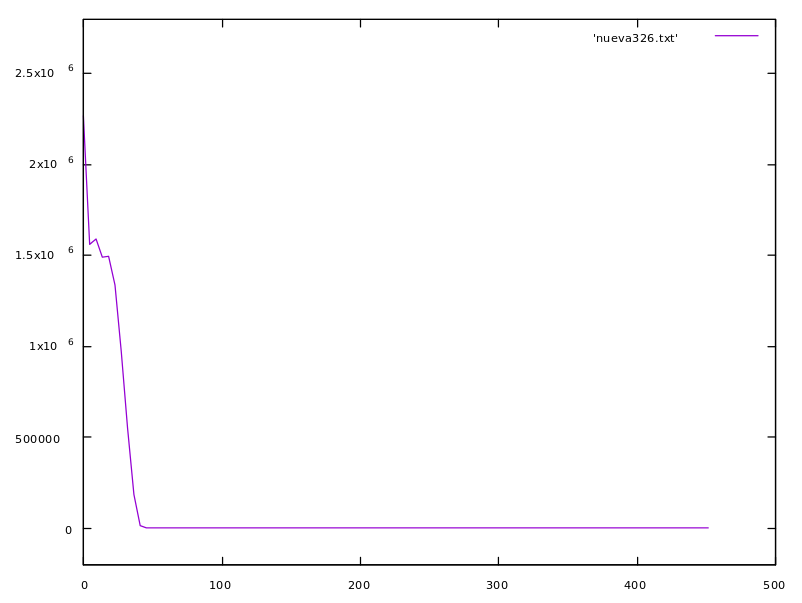
\includegraphics[scale=.5]{../imagenes/seed326.png}
    \caption{seed: 326}
\end{figure}
En cuanto tenga mis mejores soluciones, añadiré la gráfica.


\section{Conclusiones}
Aún no llego a la mejor solución con 40 ciudades y no he probado mas que un par
de veces la de 150. Tengo algunas configuraciones y con ellas algunas buenas
soluciones, por ejemplo con \textit{P=.95, EPSILON=0.0001, EPSILONP=0.001,
  L=1000, PHI=.90}, la mejor ejecución es la semilla \textit{326} y devuelve una
evaluación  de \textit{0.264213004460434}. Pero no es la mejor (la posible
mejor), así que aún me falta hacer un poco de corridas o modificar mis parámetros
. Corrí aproximadamente 1300 semillas y solo tres pasaron el 0.27, entonces, creo
que faltan muchas más pruebas, quizá modificar los datos y seguir probando. Lo
bueno es que tarda como 35 segundos en dar esa solución.
No sé si go fue la mejor opción, desde primer semestre no me sentía tan malo en
algo, pero estuvo divertido, más o menos, e interesante. Aún hay cosas que puedo
hacer o mejorar y espero hacerlas.

\bibliography{mybib}{
  \nocite{canek}
  \nocite{papadimitriou}
}
\bibliographystyle{plain}

\end{document}
